\section{User Interface}\label{sec:ui}

A standardized graphical user interface (GUI) was developed to be robust and intuitively usable by anyone. First and foremost the GUI is responsible for relaying environmental sensor and navigation data. The GUI is standardized for any ground robot that is able to traverse through a 3 degree of freedom (DOF) work space (X,Y, Theta) through an under-actuated controller. The user is able to control the robot's movement with a single virtual joystick controlling forward motion and turning. A wrapper is written to translate the joystick commands to actual motor commands. To use this GUI for other ground robot platforms, all that would need to be developed is the wrapper code that translates the joystick into movement. The second joystick is dedicated to allowing the user to manipulate the camera in real time, allowing for control over a pan-tilt unit attached to the camera base which the user can point to view regions of interest. The camera feed and joystick bandwidth is automatically adjusted and delegated based on the bandwidth that is available at a particular instance between the robotic platform and the control unit. While the control unit can be anywhere in the world, thus allowing the robot user to operate it through the internet cloud, there is better overall performance as well as lower latency in video stream and sensor data when the control unit is within the same compound as the robot. In ideal conditions, the user would be able to see and respond to any obstacle that is close by within low response time deltas, however under most conditions this isn't possible. Low level obstacle avoidance aids the user basic navigation and reduces the probability of a crash that may be unforeseen by the user. The probability of the robot crashing into an obstacle cannot be completely mitigated because of real world delays in the data stream, loss of user's focus, lapses in data due to packet loss, the camera view is facing away from the obstacle, or connection loss.

and based off of WPI's Robot Web Tools (CHRIS PUT A CITATION HERE http://robotwebtools.org/)-  

/%Another feature that has been built into the GUI is controlling based on way points instead of direct control over the robot. This allows for the user to click on the map to command the robot to navigate to the destination if possible. A 2D map is generated using SLAM from a LIDAR mounted on the robot--only differentials in the map are sent over the network. So while the initial connection may be slow, the delay during use is reasonalble. The 2D point that the user inputs is then fed into the navigation stack to attempt to reach the end goal. A third mode that the robot can be put into is pure autonomous navigation where the user can view what the robot is doing but won't have any control over the robot. The controller's multiple functionality allows for the user to pick the most appropriate mode of operation for a particular point in time, or to help the robot if it ever gets stuck. This is an important consideration when developing a GUI that is meant for long term industrial use, as all robots will eventually encounter something that they don't know how to deal with. 

As mentioned in the previous paragraph, the GUI allows the user to utilize 2 joysticks with 1 being for robot motion, and the other for camera pan-tilt motion; this 2 joystick scheme constitutes the first control mode. The GUI is designed to feature 2 more control modes. The control modes change the level of autonomy the robot exhibits during its mission. This, of course, requires for the different control modes to be hard-coded into the robot to ensure full functionality, both in terms of autonomous motion and safety of equipment in the facility being traversed. The change in control modes helps reduce the probability of mission failure or loss of robot if the control unit loses connection to the robot. The modes also change the level of involvement of the user in navigation duties, thus allowing the user to focus on higher level duties such as finding sources of contamination or thorough sterilization of the robot's local environment. This reduction of mental fatigue on the user helps increase missions success. All navigation modes utilize the map update when differentials are found, obstacle proximity alerts, and environmental sensor warnings. 

The second navigation mode provided through the GUI lets the user move the robot via way-point navigation, which is done through an interactive map of the compound that is provided to both robot and control unit prior to start of the mission. The robot is given way-point locations to reach on the interactive map by the user during the start of its mission to alleviate future bandwidth needs as the mission progresses, and distance from the control unit increases. 

\begin{figure}
\centering
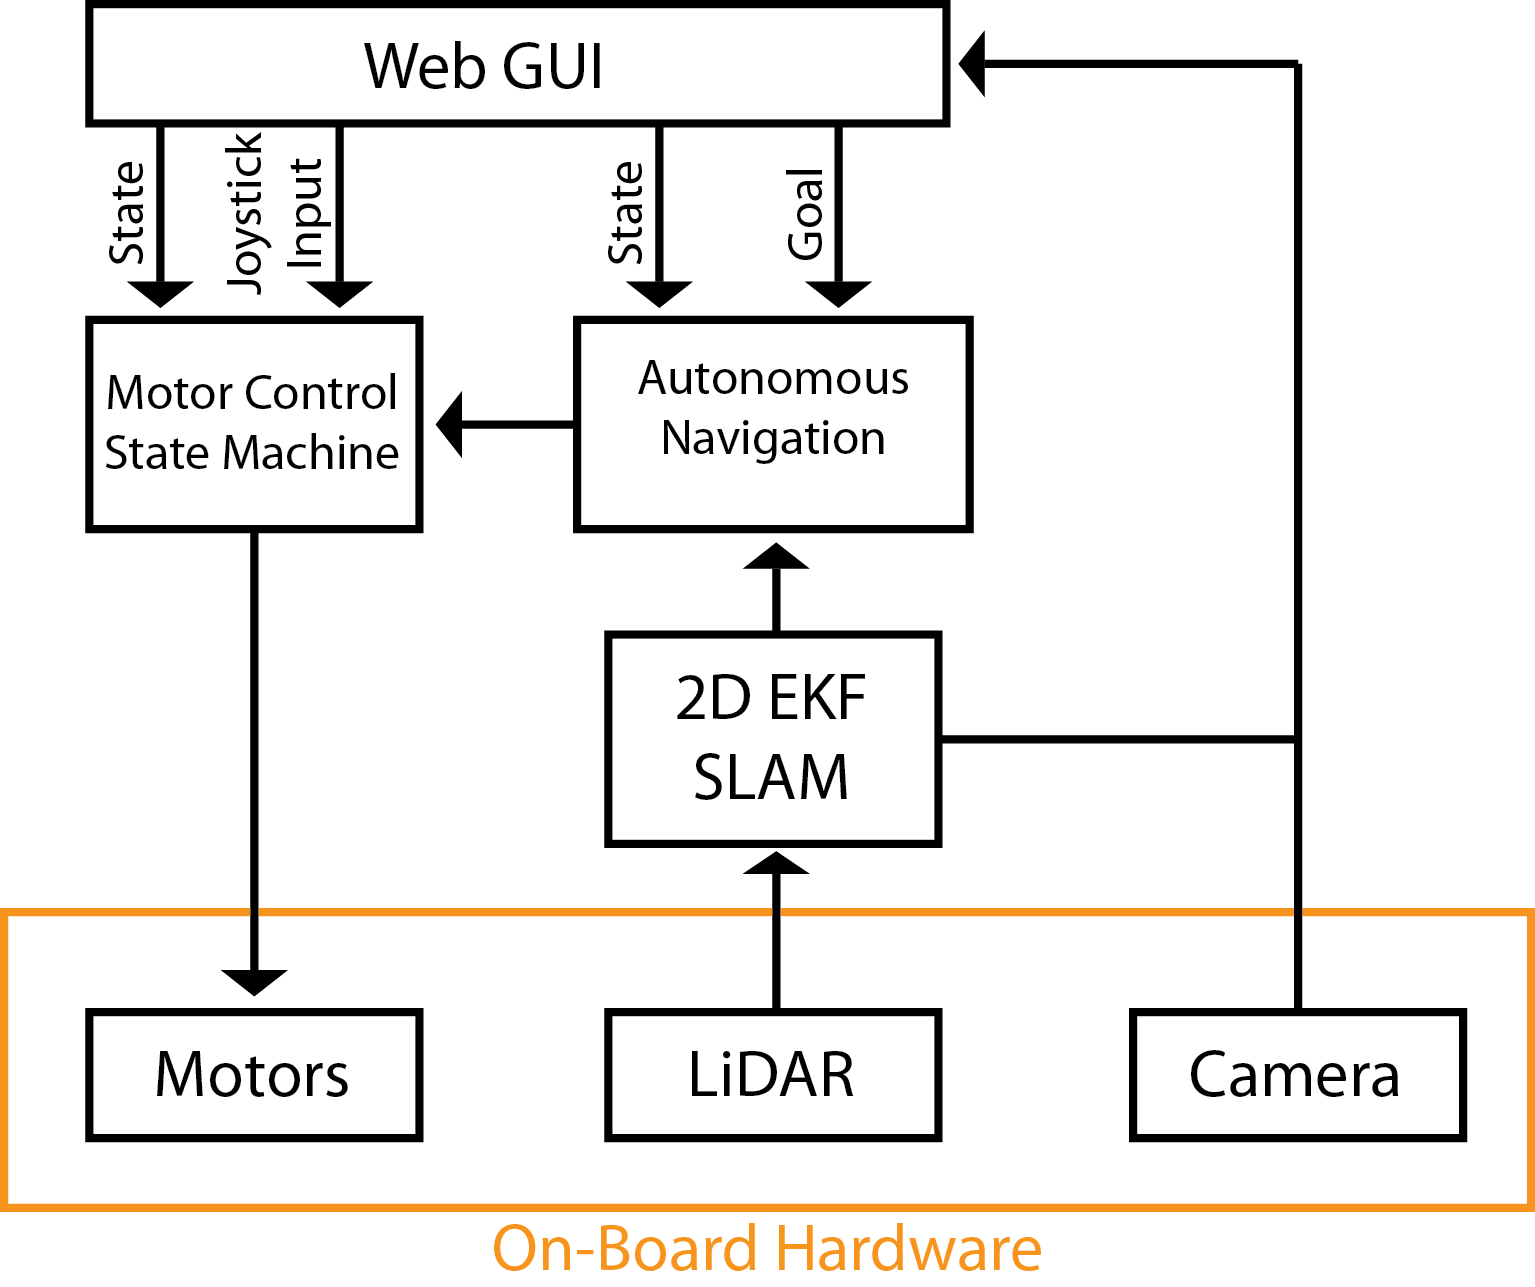
\includegraphics[width=3.4in]{pictures/Korpela_GUI.png}
\caption{System flow of individual robot interface.}
\label{gui}
\end{figure}
